\documentclass[compress]{beamer}

\usetheme{Szeged}
\RequirePackage[T1]{fontenc}
\RequirePackage[utf8]{inputenc}
\RequirePackage[frenchb]{babel}
\usepackage[babel=true,kerning=true]{microtype}
\usepackage{tikz,listings,algorithm,algorithmic}
\usetikzlibrary{automata,shapes,snakes,arrows}

\tikzstyle{every picture}=[sibling distance=3cm, shorten >=1pt, node distance=2cm,%
	>=stealth', bend angle=10, auto, initial text=]

\title[SEM IN310 - MSE]{IN310 - Modèles de systèmes embarqués}
\author[Charles Lesire]{Charles Lesire-Cabaniols (ONERA / DCSD)\\{\tt charles.lesire@onera.fr}}
\date[2010-2011]{3A-SEM - 2010-2011}

\graphicspath{{../figures/}}
\lstset{basicstyle=\tiny,tabsize=2,%frame=single,%
	emph={define,domain,requirements,strips,typing,types,predicates,
		action,parameters,precondition,vars,effect,objects,init,goal},%
	emphstyle=\bf}

\begin{document}

\begin{frame}
\titlepage
\end{frame}

\begin{frame}
\tableofcontents%[hidesubsections]
\end{frame}

%%%%% INTRODUCTION %%%%%
\section{Introduction}
\subsection{Systèmes embarqués}
\begin{frame}{Qu'est-ce qu'un système embarqué?}
\begin{itemize}
\item Un système électronique, comprenant capteurs, actionneurs, processeurs et moyens de communication, piloté par un logiciel, intégré au système qu'il contrôle et  
	\begin{itemize}
	\item soumis à diverses \structure{contraintes} : d'espace, de consommation, de temps de réponse (système temps réel), de sécurité, de  sûreté de fonctionnement ;
	\item conception conjointe "embarqueur et embarqué", mêlant différentes  \structure{spécialités}  : électronique, traitement du signal, informatique, réseaux, automatique - qui doivent se comprendre et coopérer.
	\end{itemize}
\end{itemize}	
\end{frame}
 
\begin{frame}{Qu'est-ce qu'un système embarqué?}
\begin{itemize}
\item Domaines d'application divers :
	\begin{itemize}
	\item SE orientés {\it commande} : transport (Aéronautique, Espace, Automobile, Ferroviaire, Maritime)
	\item SE orientés {\it traitement du signal/calcul} : télécom, multimédia
	\end{itemize}
\item Conception $\leadsto$ modèle :
	\begin{itemize}
	\item Comment représenter un système embarqué?
	\item Quel point de vue?\\
	$\rightarrow$ commande : Système Hybride (variables continues et discrètes)
	\end{itemize}
\end{itemize}
\end{frame}

\subsection{Types de systèmes}
\begin{frame}{Types de variables}
Le modèle mathématique d'un système est caractérisé par :
\begin{itemize}
\item la nature de la variable indépendante qui représente le \structure{temps}
\item la nature de ses \structure{variables d'état} :
	\begin{itemize}
	\item variables \structure{continues} : prennent leurs valeurs sur le domaine des réels $\mathbb{R}$
	\item variables \structure{discrètes} : prennent leurs valeurs sur un domaine représenté par un ensemble  dont le nombre d'éléments est dénombrable (ex: les  entiers naturels $\mathbb{N}$, variables booléennes)
	\end{itemize} 
\end{itemize}
\end{frame}

\begin{frame}{Types de systèmes}
\begin{itemize} 
\item \structure{Les systèmes continus} :
\begin{columns}
	\begin{column}{.7\textwidth}
		\begin{itemize}
		\item temps : variable \structure{continue} (temps dense)
		\item variables d'état \structure{continues}, évolution dictée par le temps
		\item équations algébro-différentielles $\overset{.}{x}(t)=Ax(t)+Bu(t)$, transformée de Laplace
		\item Ex : vitesse de rotation d'un moteur
		\end{itemize}
	\end{column}
	\begin{column}{.3\textwidth}
		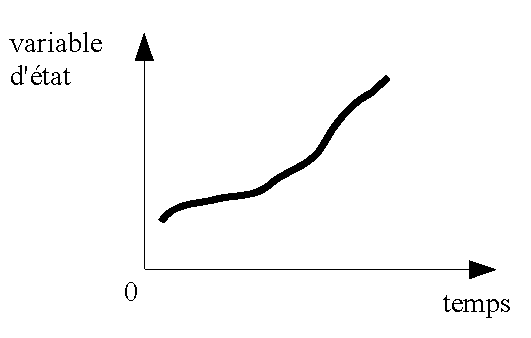
\includegraphics[width=3.7cm]{cont}
	\end{column}	
\end{columns}
\end{itemize}
\end{frame}

\begin{frame}{Types de systèmes}
\begin{itemize} 
\item \structure{Les systèmes échantillonnés} :
\begin{columns}
	\begin{column}{.7\textwidth}
		\begin{itemize}
		\item temps : variable \structure{discrète} {\scriptsize $\theta_0$, $\theta_1$ \ldots $\theta_{n-1}$ $\theta_n$, $\theta_{n+1}$ \ldots}
		\item variables d'état \structure{continues} ({\it observées} à $\theta_i$)
		\item équations différence $X_{k+1}=A_k.X_k+B_kU_k$, transformée en Z
		\item Ex : vitesse moteur controlée par un microcontroleur.
		\end{itemize}
	\end{column}
	\begin{column}{.3\textwidth}
		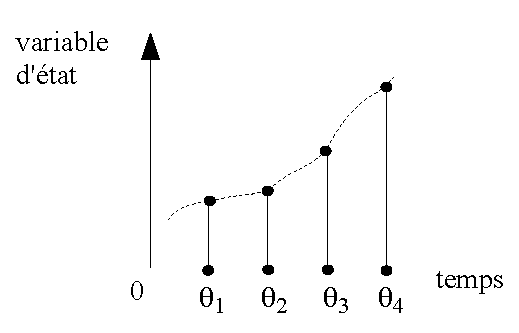
\includegraphics[width=4cm]{echant}
	\end{column}
\end{columns}
\end{itemize}
\end{frame}

\begin{frame}{Types de systèmes}
\begin{itemize} 
\item \structure{Les systèmes à événements discrets} :
	\begin{itemize}
	\item représentés par une suite d'{\it événements discrets} (ex: un plan)
	\item temps : relation de précédence
	\item variables d'état discrètes : valeur x(k+1) calculée directement à partir de x(k), sans considérer le temps (fonction des événements)
	\item automates, réseaux de Petri
	\item ex : nombre de pièces dans un système de manufacture
	\end{itemize}
\end{itemize}
\end{frame}

\begin{frame}{Types de systèmes}
\begin{itemize} 
\item \structure{Les systèmes hybrides} :
	\begin{itemize}
	\item évolution à la fois en fonction du temps  continu  et des événements discrets
	\item  variables d'état continues et  variables d'état discrètes
	\item automates hybrides, réseaux de Petri hybrides
	\item ex: contrôle de température : événement (on/off), variable continue (temperature)
	\end{itemize}
\end{itemize}
\end{frame}

\begin{frame}{Exemple}
Un réservoir qui peut être rempli ou vidé. Un même système physique, mais deux points de vue :
\begin{itemize}
\item Modélisation du niveau de liquide : $S\dot h(t)=q_i(t) - u(t).\alpha h(t)$ avec :\\
{\scriptsize $h(t)$ la hauteur de liquide, $q_i(t)$ la vitesse de remplissage, $u(t)$ l'entrée ($u(t)=0$ : valve fermée, $u(t)=1$ : valve ouverte), $S$ et $\alpha$ deux paramètres}
\item Modélisation de l'état du réservoir (vide ou plein) :\\
Espace d'état $X=$\{\emph{vide, plein}\}, contrôle $U=$\{\emph{ouvrir, fermer}\}
\end{itemize}
\end{frame}

\begin{frame}{Exemple}
Un réservoir qui peut être rempli ou vidé. Un même système physique, mais deux points de vue :
\begin{itemize}
\item Système Hybride : considérer les deux points de vue
\begin{columns}
	\begin{column}{.5\textwidth}
		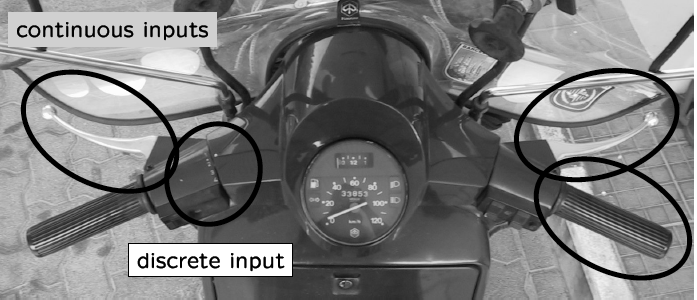
\includegraphics[width=6cm]{gear}
	\end{column}
	\begin{column}{.5\textwidth}
		\begin{itemize}
		\item Entrée discrète (rapport de vitesse)
		\item Entrées continues (frein, gaz)
		\item Etat dynamique continu (vitesse, vitesse du vent, carburant)
		\end{itemize}
	\end{column}
\end{columns}
\end{itemize}
\end{frame}

\subsection{Plan du cours}
\begin{frame}{Plan du cours}
\begin{itemize}
\item Modèles discrets
	\begin{itemize}
	\item Réseaux de Petri (C. Lesire)\\
		\small 4 C, 1 BE Tina, 2 BE Lego
	\item Automates (J. Brunel)\\
		\small 4 C, 2 BE Uppaal
	\end{itemize}
\item Modèles hybrides (C. Lesire)
	\begin{itemize}
	\item 1 C (C. Lesire)
	\item 2 BE StateFlow (F. Defaÿ)
	\end{itemize}
\end{itemize}
\end{frame}

\end{document}
